\documentclass[11pt,titlepage]{article}
\usepackage[a4paper,margin=1in]{geometry}
\usepackage[T1]{fontenc}
\usepackage[british]{babel}
\usepackage{lmodern,microtype,csquotes}
\usepackage{amsmath,booktabs,tabularx,array,multicol}
\usepackage{tikz}
\usetikzlibrary{arrows.meta,positioning}
\usepackage{graphicx,caption,setspace}
\captionsetup{labelfont=bf,textfont=it,labelsep=newline,
    justification=raggedright,singlelinecheck=false,font={small,stretch=2},skip=8pt}
\usepackage{xurl}
\usepackage[backend=biber,style=apa]{biblatex}
\addbibresource{references.bib}
\AtBeginBibliography{\interlinepenalty=10000}
\usepackage[hidelinks]{hyperref}

\setlength{\emergencystretch}{3em}
\setlength{\parindent}{1em}
\setlength{\parskip}{0.2\baselineskip}
\setlength{\columnsep}{0.3in}
\renewcommand{\dbltopfraction}{0.9}
\renewcommand{\textfraction}{0.1}
\setcounter{secnumdepth}{2}
\setcounter{tocdepth}{2}
\raggedbottom
\setlength{\belowcaptionskip}{5pt}
\newcolumntype{Y}{>{\raggedright\arraybackslash}X}
\newcommand{\visualnote}[1]{\par\vspace{4pt}{\small\raggedright\begin{spacing}{2}\noindent\textit{Note.} #1\par\end{spacing}}}

\title{How Generative AI Transforms the Duolingo User Experience:\\[0.5em]
\large What Changed, What Can Be Shown, and Whom It Serves}
\author{Artjoms Grišajevs \\ Student number: 5292573
\and Sviatoslav Zubrytskyi \\ Student number: 5375668}
\date{Applied AI --- Research Paper\\Evidence reviewed through 16 September 2026}

\begin{document}
\maketitle
\pagenumbering{roman}
\begin{multicols}{2}
\section*{Abstract}
Since 2023, generative AI has entered Duolingo through generated explanations and conversations and through content production at scale. This paper asks how these changes transform the user experience. A focused documentary review purposively selected 45 sources from a 222-record working collection and targeted retrieval. A retrospective source register records relevance, access limitations, and appraisal decisions; no exhaustive screening or learner experiment was conducted. Three sub-questions examine changes from the pre-generative app, evidence of learner effects, and enrichment versus industrialisation.

A dated timeline shows learner-facing features (Explain My Answer, Roleplay, Video Call) and production uses (AI-assisted lessons, DuoRadio, 148 new courses) developing in parallel. Field-level research reports positive but heterogeneous effects, while Duolingo-specific studies are short, mostly company-authored, and measure different confidence and performance outcomes. No inspected study directly tests motivation effects of a confirmed generative feature; demonstrated learner benefits remain unevenly supported. In the public record examined here, operational and activity indicators are documented more extensively than independent, durable learner benefits. Purposive selection and restricted source access limit this comparison, which cannot establish Duolingo's internal optimisation priorities.

\noindent\textbf{Keywords:} Duolingo; generative AI; user experience; language learning apps; learner engagement; AI-generated content.
\end{multicols}
\clearpage
\tableofcontents
\clearpage
\pagenumbering{arabic}
\twocolumn

\section{Introduction}
\label{sec:introduction}
\subsection{Reason for the Investigation}
Duolingo is a useful case for studying how generative AI changes a consumer learning product, because the company adopted it early, publicly, and on two fronts. In March 2023 it introduced Duolingo Max, a subscription tier with GPT-4-based explanations and roleplay conversations \parencite{maxLaunch}. In June 2023 it described how language models help its staff create lessons \parencite{contentProduction}, and in April 2025 it launched 148 new courses built with generative AI \parencite{courses2025}. The same technology therefore changed both what learners can do in the app and how the content they study is made.

Generative AI did not arrive in an app without artificial intelligence. Before 2023, Duolingo already personalised practice, and it used a bandit algorithm to decide which of its hand-written reminder notifications to send \parencite{freeman2023,yancey2020}. The question is therefore not whether AI entered Duolingo, but what generation adds to an experience that was already algorithmically personalised and gamified, and for whose benefit.

A large language model generates text by predicting successive continuations from the text and instructions supplied to it. This differs from the earlier adaptive selection of existing exercises: generation creates candidate wording, while selection chooses what a learner encounters. Duolingo's lesson account describes both processes and the human selection and editing of generated candidates \parencite{contentProduction}.

\subsection{Subject and Importance}
In this paper, the \emph{user experience} has three layers: the interactions available to learners, the content they encounter, and the incentives that shape when and how long they use the app. Generative AI can alter all three. A generated explanation or conversation changes the interaction; generated sentences, stories, and audio episodes change the content; and the metrics a company optimises determine which of these changes are pursued and how they are evaluated.

The topic matters beyond one company. Duolingo's management reported 23\% year-on-year growth in daily active users in the second quarter of 2026 \parencite{shareholderQ12026}, indicating expanding reach. Many of these learners study without a teacher who could correct a misleading explanation or compensate for weak generated content; if generated material is inaccurate or pedagogically shallow, self-directed learners have no external check. A 2025 review of empirical research on generative AI in language learning found the evidence concentrated in higher-education and English-as-a-foreign-language settings rather than self-directed app use \parencite{liReview2025}. Assessing this case therefore requires distinguishing documented product changes from demonstrated learner benefits.

\subsection{Research Questions and Objective}
The inspected field review maps language-learning research broadly, while product announcements document changing features; neither alone connects a dated Duolingo version to attributable learner outcomes \parencite{liReview2025,maxLaunch,duocon2024}. This review addresses that gap by linking the product chronology to source-specific evidence and its limitations. The objective is to describe the changes, assess learner-effect claims, and examine what public reporting can establish about learner and company outcomes.

\noindent\textbf{Main research question}

How does generative AI transform the Duolingo user experience?

\noindent\textbf{Sub-questions}
\begin{enumerate}
    \item What generative-AI features has Duolingo deployed since 2023, and how do they differ from the pre-generative user experience?
    \item What evidence exists that these features change learners' motivation, confidence, and engagement, and how much of it concerns Duolingo specifically rather than being inferred from the wider generative-AI literature?
    \item Does generative AI enrich the Duolingo experience or industrialise it, and whose outcomes is the system optimised for?
\end{enumerate}

In RQ3, \emph{capability enrichment} means an expansion of available practice or support, while \emph{industrialisation} means higher-volume, lower-cost content production or interaction delivery; these terms are defined operationally in \S\ref{sec:rq3}. The sub-questions build on each other: RQ1 describes the change, RQ2 appraises the evidence about its effects, and RQ3 uses both to construct an argument.

\subsection{Scope and Reading Guide}
The review covers Duolingo's consumer language courses from 2023 to September 2026. It includes both learner-facing generative features and generative content production, because both shape what learners experience. The Duolingo English Test, the mathematics, music, and chess courses, and labour relations are excluded. Technical architecture is discussed only where it explains the experience. Section~\ref{sec:method} explains how sources were selected and appraised, Section~\ref{sec:results} answers the three sub-questions in turn, and Section~\ref{sec:conclusion-discussion} answers the main question, evaluates the method, and makes recommendations.

\section{Method}
\label{sec:method}
\subsection{Design, Population, and Sample}
This study is a focused documentary review. Its population is the public record on generative AI in Duolingo: company announcements, product and engineering documentation, investor communications, research about Duolingo, and research syntheses on generative AI in language learning. No learners were recruited, no accounts were tested, and no model outputs were scored. The unit of analysis is a document, and the review compares what documents claim with the kind of evidence they supply.

A pre-existing collection of 222 annotated Duolingo/AI records served as a discovery frame, supplemented by targeted retrieval. Of those 222 records, approximately 90 were assessed for relevance against the sub-questions; the remainder were excluded early as duplicates, non-English items, or records outside scope (English Test, non-language courses, pure labour-relations coverage). Of those assessed, 45 were retained as the cited sample, selected purposively for a dated product change, a relevant learner outcome, a research synthesis, or an explicitly attributed interpretation bearing on RQ1--RQ3. Baseline documents before 2023 were retained to identify what generation changed; unverified feature exposure was retained only as general-app context. These are the scope rules used in this review, not a claim that all 222 records underwent full-text screening.

Both authors contributed to retrieval and selection. Coding against the instruments in \S\ref{sec:instruments} was conducted by a single rater per source; no independent duplicate extraction was performed. This is disclosed as a reliability limitation in \S\ref{sec:conclusion-discussion}.

The accompanying research supplement, \nolinkurl{method-supplement.md} and \nolinkurl{current-source-register.csv}, reconstructs the selection and appraisal trail for every cited key. It records inventory matches, retrieval provenance, RQ relevance, inclusion rationale, access, locators, and claim limits. This register was assembled retrospectively on 16 September 2026 from the manuscript, inventory, and saved research logs; this retrospective character is a limitation (\S\ref{sec:conclusion-discussion}). It documents the final selection; it cannot recover unrecorded search results or exclusion decisions.

\subsection{Data Collection}
Retrieval used company research, blog, and investor pages, publisher and author-hosted records, and web searches for exact titles, DOIs, and feature/outcome combinations. Saved September 9--14 logs include queries such as \texttt{Duolingo "Video Call" confidence engagement study 2026 2025}, \texttt{"Duolingo Max" "Roleplay" "study" confidence independent}, \texttt{Duolingo generative AI "lesson" quality evaluation}, \texttt{Duolingo "DuoRadio" AI scale}, \texttt{"Explain My Answer" Duolingo effectiveness}, and \texttt{Duolingo AI "self-efficacy" OR "motivation" OR "engagement"}. These targeted searches were supplemented by claim-specific checks on 16 September. The supplement separates those new checks from historical records; no complete database export or timestamped screening history is available.

Claims were checked against accessible original-source passages. Complete text, selected original passages, abstracts, and indexed passages are distinguished in the register. For example, the Japanese Video Call report was available through indexed original passages, whereas detailed appraisal of the Li et al. meta-analysis and two working papers remains abstract-limited \parencite{kittredge2025video,liMeta2025,harrison2025,espinosa2026}. Inaccessible design details were left unresolved rather than taken from inventory annotations.

Dates were recorded at event level. An announcement, a platform rollout, a later technical description, and a change in subscription access were treated as separate events, because a study can only evaluate the version that existed when its data were collected. Live webpages can be edited after publication, so dated releases and filings were preferred for timing claims.

\subsection{Instruments}
\label{sec:instruments}
Four instruments were used.

The first instrument was a \emph{dated timeline}, recording event date and type (announcement, rollout, technical description, or access change), whether the event belongs to the interaction track or the production track, and the source. Because a study can only evaluate the version of the app that existed when its data were collected, events are dated individually rather than grouped by feature.

The second instrument was a \emph{source register} applied to each cited document, recording population, confirmed exposure, comparison, measure and timing, source relationship (company-authored, external, or mixed), and permitted inference. Its codebook defines a confirmed feature as one explicitly named in the inspected intervention description; the app name or publication year alone is insufficient. External authorship is recorded separately from design quality, and external reporting of a company statement remains company-reported evidence. Unreported information is coded as unresolved, never as evidence of its absence.

The third instrument was an \emph{outcome coding scheme} derived from the sub-questions. Each finding was assigned to one of seven outcome categories: motivation (reasons for persisting), self-efficacy (perceived task capability), willingness to communicate (readiness to communicate), post-use confidence perceptions, behavioural participation, emotional/cognitive engagement, and language performance. Pre/post change, post-only perceptions, and aggregate trends are not interchangeable and were never combined.

The fourth instrument was an \emph{evidential criterion} applied consistently throughout the analysis: four appraisal questions governed every claim drawn from a source.
\begin{enumerate}
    \item Does the confirmed exposure match the claimed feature?
    \item Does the comparison support attribution to that feature?
    \item Does the measure capture the stated outcome?
    \item Does the sample support generalisation beyond those studied?
\end{enumerate}
This distinction between what a design can and cannot show is the principal safeguard against overstating the evidence.

\noindent\textbf{Worked example.} The Japanese Video Call report \parencite{kittredge2025video} is coded as follows. (1)~Exposure: confirmed --- the intervention description names Video Call and the study randomly assigned learners to use it. (2)~Comparison: partial --- a regular-lesson control exists, but weekly adherence exclusions removed more Video Call users (263 of 329 analysed vs.\ 304 of 329), and mean practice time differed (13.05~h vs.\ 9.11~h), so the comparison cannot isolate conversation format from practice dose. (3)~Measure: the Versant Speaking and Listening Test captures spoken performance; the adapted willingness-to-communicate scale and post-use confidence items are self-report and do not measure change in the same sense. (4)~Generalisation: restricted --- the sample consists of Japanese learners of English selected for adherence; results need not generalise to other languages, proficiency levels, or non-adherent users. Source relationship: company-authored. Permitted inference: a short-term speaking advantage under these conditions, with stable willingness to communicate and neutral confidence perceptions; not a general confidence or motivation effect.

\subsection{Analysis}
For RQ1, events were ordered and compared with the pre-generative baseline. For RQ2, specificity (confirmed feature, general Duolingo, or other AI settings) and source relationship separated direct evidence from contextual inference. For example, the Japanese Video Call report was coded as confirmed exposure, company-authored, and stratified random assignment. Its 30-day comparison supports a short-term speaking finding, but post-assignment exclusions and unequal practice time restrict attribution. Pre/post willingness to communicate and post-use confidence perceptions were entered separately, not combined into a confidence-change estimate \parencite{kittredge2025video}.

For RQ3, a ledger contrasts new practice capabilities with throughput, cost, and activity indicators, keeping demonstrated learner benefits separate. Ambiguous exposure remains contextual; overlapping reviews or company summaries are not counted as independent replications. This is a qualitative synthesis: the prevalence of topics in purposively selected documents cannot estimate all available evidence or reveal internal objective weights.

\subsection{Justification of Methodological Choices}
A documentary review suits the questions because the relevant changes are publicly documented and a controlled learner study was not feasible within the available time. Separating specificity from independence prevents two common errors: treating positive field-level findings as proof for one product, and dismissing company research merely because of its authorship. Company documentation is used to establish what was offered and when, but not whether it worked. No quality score or pooled estimate was calculated, because the included studies differ too much in design and outcome to be combined meaningfully.

\clearpage
\section{Results}
\label{sec:results}

\subsection{RQ1: What Changed, and Against What Baseline?}
\label{sec:rq1}
\subsubsection{The Pre-Generative Baseline}
Before March 2023, Duolingo was already an AI-supported, gamified app. Its January 2023 method report emphasises structured activity, personalisation, and sustained participation \parencite{freeman2023}. A systematic review of Duolingo research from the app's 2012 public release to early 2020 shows that researchers had long approached it through its gamification \parencite{shortt2023}. Engagement was also algorithmically optimised. A bandit algorithm chose among hand-written reminder templates and counted a notification as successful when the learner completed a lesson within two hours; in deployment it raised daily active users by 0.5\% and new-user retention by 2\% \parencite{yancey2020}.

Studies of general app use help characterise the baseline. \textcite{liBonk2025}, whose article was submitted in 2022, interviewed ten self-directed learners who combined Duolingo with other resources. A six-week study of 20 Chinese Year~8 students found that motivation for app activities could transfer to broader motivation for learning English \parencite{zeng2024}. Other studies compared Duolingo with HelloTalk over five weeks \parencite{zhao2024} or followed 80 EFL learners over two months \parencite{ouyang2024}. None establishes exposure to a generative feature. More broadly, a review of 18 studies associated learner independence with AI tools combined with explicit self-regulation instruction and scaffolding \parencite{mohebbi2025}.

Together, these sources characterise the baseline as pre-authored exercises in an adaptive sequence, correctness-based feedback, and gamified mechanisms that encourage learners to return. Learners could be motivated and practise regularly, but their contributions were largely confined to formats written in advance by course designers. This is an analytical characterisation, not a claim that the earlier app offered no speaking practice or explanations.

\subsubsection{A Dated Timeline in Two Tracks}
Table~\ref{tab:timeline} orders the changes since 2023. Two tracks are visible. The \emph{interaction track} consists of features that learners use directly; the \emph{production track} consists of uses of generative AI that change how content is made before learners see it.

\begin{table*}[t]
\centering
\small
\caption{Generative-AI Changes to the Duolingo Experience by Date and Track}
\label{tab:timeline}
\begin{tabularx}{\textwidth}{@{}>{\raggedright\arraybackslash}p{0.13\textwidth}>{\raggedright\arraybackslash}p{0.11\textwidth}YY@{}}
\toprule
Date & Track & Change & Consequence for the experience \\
\midrule
11 Jan 2023 & Baseline & Method report on structured, personalised, gamified learning \parencite{freeman2023} & Reference point for later change \\
14 Mar 2023 & Interaction & Duolingo Max launches Explain My Answer and Roleplay with GPT-4 \parencite{maxLaunch} & Contextual explanations and scenario conversations for subscribers \\
22 Jun 2023 & Production & Account of a model drafting lesson exercises for human selection \parencite{contentProduction} & Faster exercise creation; designers select and edit \\
Late 2023--Mar 2025 & Production & Late-2023 DuoRadio launch; 2024 automation hackathon; scaling account published in March 2025 \parencite{duoradio} & Listening episodes grow from 300 to 15,000+ \\
24 Sep 2024 & Interaction & Video Call with Lily announced \parencite{duocon2024} & Open spoken conversation with an AI character \\
16 Jan 2025 & Interaction & Video Call extended to Android \parencite{android2025} & Wider device availability \\
30 Apr 2025 & Production & 148 new courses built with generative AI \parencite{courses2025} & Course offer doubled, mainly at beginner level \\
29 Dec 2025 & Interaction & Explain My Answer announced as free from 1 January 2026 \parencite{explainAccess2025} & Explanations move from a paid tier to free users \\
May--Aug 2026 & Interaction & Video Call extended to Super subscribers \parencite{shareholderQ12026,earnings2026} & Conversation practice reaches a cheaper tier \\
\bottomrule
\end{tabularx}
\visualnote{Authors' chronology from the cited sources. Dates distinguish announcements, documentation, and access changes. Availability varied by platform, course, and subscription. AI = artificial intelligence.}
\end{table*}

The interaction track began with Explain My Answer and Roleplay in March 2023 (Table~\ref{tab:timeline}). In Explain My Answer, a learner who answers incorrectly taps to receive a generated paragraph explaining why the answer was wrong and what the correct answer means in context \parencite{explainFree}. Roleplay presents a scenario (ordering in a restaurant, booking a hotel) and a character; the learner types responses in the target language, and the system replies using specialised prompts containing the scenario, character, learning objective, and proficiency level, with application logic managing the exchange \parencite{roleplayDesign}.

Video Call extends the interaction to speech. The learner sees Lily, an animated character, on screen and holds a spoken conversation in real time. Conversations are structured around a topic (a travel plan, a recipe, a weekend), and the system can ask follow-up questions, respond to what the learner says, and incorporate facts extracted from earlier calls \parencite{henry2025,videoCall}. A call typically runs for several minutes of open conversation, unlike the fixed-answer exercises in regular lessons. When the call ends, the learner receives a summary of the conversation. Designers specify Lily's character and language level, while a program structures the exchange \parencite{henry2025}. Guided calls with Falstaff add on-screen suggested phrases, translations, and feedback for beginners, so that a learner who cannot yet produce a full sentence can still participate \parencite{falstaff}.

The production track ran in parallel. Figure~\ref{fig:workflows} contrasts designer-led lesson creation with the documented Video Call process. In the lesson example, a model drafts ten exercises and a designer selects and edits three \parencite{contentProduction}. DuoRadio followed a different route: after its late-2023 launch, a 2024 hackathon developed curriculum-based script generation and designer-written evaluation prompts. The company reports expansion from 300 to 15,000+ episodes and 2 to 25+ courses, with 99\% cost savings and daily sessions rising from 500,000 to 5 million \parencite{duoradio}. Proficiency-controlled text generation has also been researched, without establishing product deployment \parencite{malik2024}. The 148 courses released in April 2025 mainly targeted beginners and included Stories and DuoRadio \parencite{courses2025,malikTechcrunch2025}.

\begin{figure*}[t]
\caption{Documented Workflows for Lesson Production and Video Call}
\label{fig:workflows}
\centering
% Original schematic based on Henry (2023, 2025); see the figure note in main.tex.
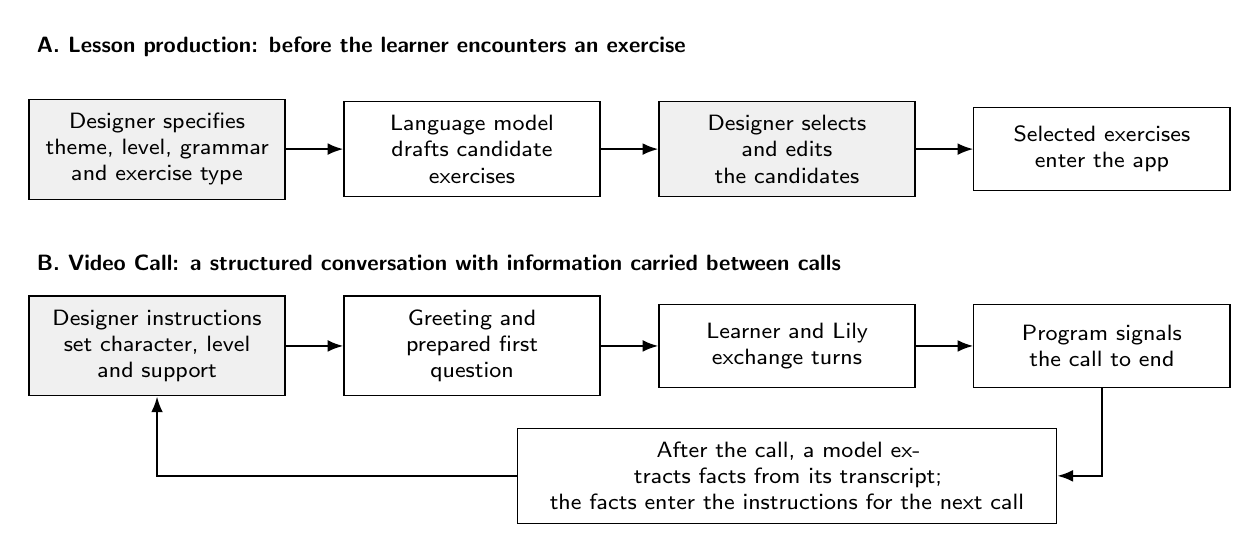
\begin{tikzpicture}[
    box/.style={draw,align=center,text width=2.9cm,minimum height=1.05cm,
        font=\sffamily\footnotesize,inner sep=5pt},
    flow/.style={-{Latex[length=2mm]},thick},
    label/.style={font=\sffamily\footnotesize,align=left}]
\node[label,anchor=west] at (-1.65,1.3) {\textbf{A. Lesson production: before the learner encounters an exercise}};
\node[box,fill=black!6] (design) at (0,0) {Designer specifies\\theme, level, grammar\\and exercise type};
\node[box] (draft) at (4,0) {Language model\\drafts candidate\\exercises};
\node[box,fill=black!6] (edit) at (8,0) {Designer selects\\and edits\\the candidates};
\node[box] (lesson) at (12,0) {Selected exercises\\enter the app};
\draw[flow] (design) -- (draft);
\draw[flow] (draft) -- (edit);
\draw[flow] (edit) -- (lesson);

\node[label,anchor=west] at (-1.65,-1.45) {\textbf{B. Video Call: a structured conversation with information carried between calls}};
\node[box,fill=black!6] (system) at (0,-2.5) {Designer instructions\\set character, level\\and support};
\node[box] (start) at (4,-2.5) {Greeting and\\prepared first\\question};
\node[box] (chat) at (8,-2.5) {Learner and Lily\\exchange turns};
\node[box] (close) at (12,-2.5) {Program signals\\the call to end};
\node[box,text width=6.5cm,minimum height=0.8cm] (memory) at (8,-4.15)
    {After the call, a model extracts facts from its transcript;\\the facts enter the instructions for the next call};
\draw[flow] (system) -- (start);
\draw[flow] (start) -- (chat);
\draw[flow] (chat) -- (close);
\draw[flow] (close.south) |- (memory.east);
\draw[flow] (memory.west) -| (system.south);
\end{tikzpicture}

\visualnote{Original schematic based on \textcite{contentProduction,henry2025}. Arrows represent described workflow and information flow, not effectiveness. Panel A concerns lesson exercises, not the separate automated DuoRadio pipeline.}
\end{figure*}

Explain My Answer was announced as free from 1 January 2026 \parencite{explainAccess2025}, and Video Call began reaching Super in 2026 \parencite{shareholderQ12026}. Management linked wider access to per-call costs falling from about \$0.30 to under \$0.01 following a shift towards open-source models \parencite{shareholderQ12026,earnings2026}.

\subsubsection{How the Experience Differs}
Compared with the baseline, the interaction track introduces three changes. First, generated explanations add a context-specific account of \emph{why} an answer is correct or incorrect to existing correctness feedback. Second, practice moves from selecting among pre-authored options to producing open responses that the system answers. In Roleplay and Video Call, the learner's own utterance shapes the next turn, which fixed exercise formats cannot do. Third, the experience becomes partly persistent, because facts from earlier calls can shape later conversations \parencite{henry2025}. Guidance adds a fourth, less obvious change. Because guided calls offer suggested phrases and translations \parencite{falstaff}, a beginner can produce a first turn that would otherwise be out of reach, but a learner who repeatedly copies suggestions can also complete a conversation without producing language independently. Completing a task therefore means something different in a guided call than in a fixed exercise, and it cannot by itself show what the learner can do.

The production track changes the experience differently. Learners do not choose generated content; they meet it as ordinary lessons, stories, or episodes. The change is therefore largely invisible at the moment of use, but it determines which courses exist, how much listening material is available, and how quickly new content appears. Even researchers studying generated lessons could not confirm which of the lessons their participants had seen were generated \parencite{catalan2026}.

Several elements did not change. Lessons remain structured and gamified, streaks and reminders still encourage daily return, and the generative features operate within designer-written instructions rather than as unrestricted chatbots \parencite{roleplayDesign,henry2025}. The transformation is thus an extension of an existing adaptive, gamified product, not its replacement.

\subsubsection{Why the Dates Matter}
Timing limits what RQ2 can establish. Data collected before the Max launch cannot evaluate its generative features, and 2023 data cannot evaluate Video Call (Table~\ref{tab:timeline}). General app use is not confirmed feature exposure. Access conditions also matter: the self-efficacy study collected data in late 2023 from subscribers and learners given access for the study \parencite{kittredge2025self}. Its findings need not generalise to the later free-access population. Each study is interpreted against its feature version and access conditions.

\subsection{RQ2: What Can Be Shown About the Effects on Learners?}
\label{sec:rq2}
\subsubsection{Outcomes and Evidence Standards}
Three outcome families are examined. \emph{Motivation} concerns reasons for persisting. Confidence-related reports are distinguished by construct and timing: task-specific \emph{self-efficacy} concerns perceived capability; \emph{willingness to communicate} concerns readiness to communicate; and \emph{post-use confidence perceptions} do not by themselves measure change. None is a proficiency score. \emph{Engagement} distinguishes behavioural participation, emotional involvement, and cognitive investment \parencite{loEngagement2024}. Activity can increase without deeper engagement, and perceived capability can differ from performance. Each finding is classified by confirmed exposure, measure, and source relationship.

\subsubsection{Field-Level Evidence Is Substantial}
Research on generative AI in language learning has grown quickly. A systematic review of 144 empirical articles from 2023 and 2024 found that 86.7\% of studies took place in higher education and 86.1\% in English-as-a-foreign-language contexts. Writing was the most frequent focus, at 42.4\%, while speaking, listening, and reading received less attention, and longitudinal studies were scarce \parencite{liReview2025}.

Quantitative syntheses report positive averages. A meta-analysis of 41 experimental or quasi-experimental studies with 3,515 participants reports improved second-language acquisition; its accessible abstract does not name the effect-size metric or permit detailed comparator and bias appraisal, so no numerical magnitude is adopted here \parencite{liMeta2025}. A second synthesis of 51 studies required comparison groups and reported positive language and affective--cognitive outcomes. Its overall random-effects estimate was Hedges' \(g = 0.81\) (95\% CI [0.61, 1.02]), with very high heterogeneity (\(I^2 = 98.4\%\)) and significant small-study effects. Positive sensitivity findings do not remove those concerns \parencite[Sections 3.1, 4.3]{saarela2026}. A review of 25 task-based studies with 2,431 participants identified AI literacy, planning, and assessment as potential moderators \parencite{liTask2026}. For broader AI-guided personalisation, 61 samples from 17 projects yielded a between-group \(d = 0.39\) and within-group \(d = 1.18\); these estimate different comparisons and are not generative-feature effects \parencite{lee2024}.

These results support the plausibility of generative conversation and feedback, but do not predict the benefit of a Duolingo feature. The syntheses combine different tools, comparators, populations, and teacher support. Moderator associations, including larger effects in informal settings or productive skills \parencite{saarela2026}, suggest hypotheses for app studies rather than establish transfer to Duolingo. Reviews overlap, so their participant totals cannot be added. A positive pooled average also does not show that every intervention helps or that benefits persist after use ends.

\subsubsection{Duolingo-Specific Evidence Is Thin}
The closest evidence comes from Duolingo itself. \textcite{kittredge2025self} studied self-efficacy after one month of access to Roleplay and Explain My Answer, with data collected between 30 August and 17 November 2023. Final analyses included 153 existing subscribers and 232 learners newly given access. Significant improvement was found for one of seven analysed self-efficacy items in the existing-user cohort and for six in the new-access cohort. There was no control group without the features, seven of seventeen collected items were selected for analysis, six-point responses were dichotomised, and feature-use counts did not significantly predict post-survey self-efficacy. Usage requirements selected adherent participants, and all authors were affiliated with Duolingo.

A company report stratified and randomly assigned 658 Japanese learners of English to 30-day Video Call or regular-lesson conditions. Speaking analyses included 567 learners using the Versant Speaking and Listening Test; 558 entered survey analyses. The report found a small speaking advantage, stable pre/post willingness to communicate on an adapted nine-item scale, and neutral post-only confidence perceptions. Random assignment strengthens the design, but weekly adherence exclusions were unequal, and mean total learning time over 30 days differed: 13.05 hours for analysed Video Call users versus 9.11 for regular-lesson users. The comparison therefore does not isolate conversation format from practice dose \parencite[Sections 2.2--2.3, Tables 3--4]{kittredge2025video}. A later summary reports better speaking and higher confidence for English speakers learning Spanish with Lily, but sample, assignment, and instruments are incompletely reported \parencite{videoResearch}. Guided Falstaff calls are associated with better spoken translation of practised phrases, an outcome narrower than general speaking or confidence \parencite{falstaffResearch}. Reported average words spoken per Video Call user more than doubled over a year \parencite{shareholderQ12026}; changing versions and populations limit this to a participation indicator.

Figure~\ref{fig:video-sample} makes the unequal analysis inclusion in the Japanese study visible: 263 of 329 learners in the Video Call condition entered the speaking analysis, compared with 304 of 329 in the regular-lesson condition. These are analysis-inclusion proportions, not natural app-retention rates; the conditions imposed different usage requirements.

\begin{figure*}[t]
\caption{Analysis Samples in the 30-Day Video Call Study}
\label{fig:video-sample}
\centering
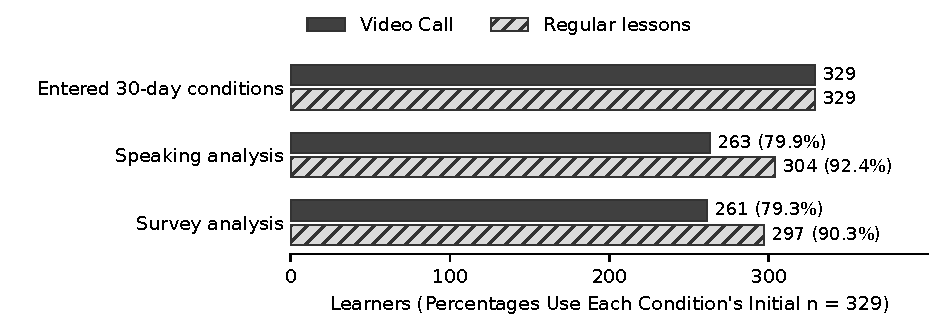
\includegraphics[width=\textwidth]{figures/video-sample.pdf}
\visualnote{Original chart of counts from \textcite[Figure~2, p.~5]{kittredge2025video}; indexed original inspected. Percentages divide each analysis count by 329. Exclusions and missing follow-up data both reduce the samples.}
\end{figure*}

Independent research is scarcer. \textcite{harrison2025} reviews Video Call alongside other conversational tools, but the accessible abstract identifies it as a technology review rather than a learner study. \textcite{catalan2026} surveyed five software engineers in the Philippines who were learning Korean. They found general scenarios helpful for grammar and vocabulary, but rarely encountered work-related scenarios and wanted more personalised content; the authors did not verify which lessons were generated. \textcite{xu2025} compare Duolingo with ChatGPT on motivation, enjoyment, critical thinking, and autonomy, but the accessible material does not establish which Duolingo features or version participants used, so the study cannot be treated as evidence about generative features.

\subsubsection{What Comparable Studies Add}
Studies outside Duolingo help interpret the distinction between perceived and demonstrated capability. \textcite{wangConversation2024} compared three classes of 33 Chinese undergraduates practising with a teacher and peers, a text-and-voice chatbot, or an avatar-based generative chatbot. The avatar condition improved willingness to communicate and self-perceived competence and reduced anxiety relative to the teacher-and-peer group, without a significant speaking-performance advantage. Different instruments and populations prevent a direct effect comparison with the Japanese Video Call study; non-significance does not establish equivalence. \textcite{celik2025} reported higher speaking self-efficacy after eight weeks with 44 university learners, but convenience sampling and additional practice and training limit attribution to ChatGPT. Both studies support measuring self-report and performance separately, rather than validating a Duolingo effect.

The setting also matters. In a study of 60 learners using a generative chatbot, those with a teacher present reported higher emotional and agentic engagement than those without, whereas behavioural and cognitive engagement did not differ significantly \parencite{liTeacher2026}. Most field-level studies take place in classes where teachers can explain feedback and hold learners accountable, while Duolingo learners typically practise alone. Benefits observed in supported classrooms cannot be assumed to reproduce in unsupervised app use.

\begin{table*}[t]
\centering
\small
\caption{Evidence on Learner Effects by Specificity and Independence}
\label{tab:evidence}
\begin{tabularx}{\textwidth}{@{}>{\raggedright\arraybackslash}p{0.18\textwidth}>{\raggedright\arraybackslash}p{0.16\textwidth}>{\raggedright\arraybackslash}p{0.20\textwidth}>{\raggedright\arraybackslash}p{0.09\textwidth}Y@{}}
\toprule
Source & Specificity; authorship & Design and sample & Outcome & What it can show \\
\midrule
\textcite{kittredge2025self} & Confirmed feature; company & Pre/post, 153 and 232 learners, one month, no control & SE & Some self-efficacy items improved among selected users \\
\textcite{kittredge2025video} & Confirmed feature; company & Randomised; 30 days; analysed: 567 speaking, 558 survey & W, C, P & Speaking advantage; stable willingness to communicate; neutral post-use confidence; unequal exclusions/time \\
\textcite{videoResearch}; \textcite{falstaffResearch} & Confirmed feature; company summaries & Sample and assignment incompletely reported & C, P & Positive summaries with limited appraisal \\
\textcite{shareholderQ12026} & Confirmed feature; company filing & Aggregate usage statistic & B & Participation, not learning \\
\textcite{catalan2026} & Generation unverified; external & Survey of five learners & Views & Learner views, no effect estimate \\
\textcite{harrison2025}; \textcite{xu2025} & Feature confirmed or uncertain; external & Review; app/ChatGPT comparison & --- & Context; no attributable feature outcome \\
\textcite{liMeta2025}; \textcite{saarela2026} & Field level; external & Meta-analyses of 41 and 51 studies & P, A & Positive but heterogeneous averages \\
\textcite{liReview2025} & Field level; external & Review of 144 studies & Mapping & Evidence skewed to higher education and writing \\
\bottomrule
\end{tabularx}
\visualnote{SE = self-efficacy; W = willingness to communicate; C = confidence perceptions (timing differs by source); B = behavioural engagement; P = performance; A = affective--cognitive outcomes; --- = no attributable outcome. Rows are not independent replications; samples must not be added.}
\end{table*}

\subsubsection{Motivation, Confidence, and Engagement Compared}
Table~\ref{tab:evidence} maps this evidence against specificity and authorship. The pattern differs sharply by outcome, and one absence is itself a finding.

\emph{Motivation} is the clearest gap: no inspected study directly tests motivation effects of a confirmed Duolingo generative feature. Evidence that Duolingo supports motivation comes from general app use before the generative features existed \parencite{zeng2024}, and evidence that generative AI supports affective outcomes comes from outside Duolingo \parencite{saarela2026}. The claim that Duolingo's generative features motivate learners is therefore an inference combining two bodies of evidence, neither of which tests it directly. This is not a failure to find an effect; it is the absence of a study that could detect one.

For \emph{confidence}, direct evidence exists but is mixed. Selected Roleplay and Explain My Answer users reported higher self-efficacy on some items, without a control group \parencite{kittredge2025self}; Japanese learners showed stable willingness to communicate and neutral confidence perceptions despite a performance benefit \parencite{kittredge2025video}; and a less detailed summary reports higher confidence among Spanish learners \parencite{videoResearch}. The mix is itself informative: confidence and performance need not move together.

For \emph{engagement}, the only direct record concerns behavioural participation: spoken words per user increased \parencite{shareholderQ12026}. This shows that users who remain active speak more, but it cannot distinguish deeper engagement from longer sessions. Emotional and cognitive engagement with the generative features --- whether learners interpret explanations, repair misunderstandings, or merely consume generated responses --- is not measured in the inspected sources. These dimensions are not company secrets withheld from the public record; they are constructs that require purpose-built instruments and have simply not been studied for confirmed Duolingo features. Field research advises caution: evidence on cognitive engagement with ChatGPT is broad but weak \parencite{loEngagement2024}, and in a small case study favourable reactions to ChatGPT feedback did not ensure that learners used the feedback effectively \parencite{yan2024}.

\subsubsection{The Evidence Asymmetry}
The central finding of RQ2 is an asymmetry in the inspected record. Field-level syntheses report positive but heterogeneous effects. At Duolingo level, the evidence consists of a peer-reviewed company self-report study, a company report with mixed outcomes, shorter company summaries, an aggregate usage statistic, and small or access-limited external papers. The two detailed direct studies follow learners for about a month; the shorter summaries do not permit equivalent design appraisal. No independent controlled feature evaluation was identified in this selection, which does not establish that none exists.

The design details of the direct studies further limit what their positive results mean. When learners must use a feature regularly before follow-up, the results describe those who kept using it, not everyone who was offered it; for engagement, the learners who stop are part of the outcome. Converting six-point ratings into two categories discards differences in the strength of confidence, and a statistically significant change on a questionnaire item is not necessarily a meaningful change for a learner. Equally, the non-significant association between feature use and self-efficacy does not show that use is irrelevant; it shows that this design detected no association.

This asymmetry does not show ineffectiveness. The company reports include neutral perceptions and a non-significant usage association as well as positive findings. The answer to RQ2 is that selected users show some short-term self-efficacy and speaking gains, while reported speech volume indicates participation. Motivation and deeper engagement remain unmeasured in the inspected direct record. Wider findings support plausible benefits, but cannot establish their magnitude, durability, or distribution among Duolingo users.

\subsection{RQ3: Enrichment or Industrialisation?}
\label{sec:rq3}
\subsubsection{Two Readings of the Same Change}
Here, \emph{capability enrichment} means an expansion of available practice or support, established through documented affordances and access. \emph{Demonstrated learner benefit} requires measured outcomes and an appropriate comparison; availability alone is insufficient. \emph{Industrialisation} means higher-volume, lower-cost content production or interaction delivery, assessed through operational indicators. It does not imply poor quality. Table~\ref{tab:ledger} contrasts these two readings by area, and Figure~\ref{fig:tracks} connects them to the outcomes visible in the inspected record.

\begin{table*}[t]
\centering
\small
\caption{Enrichment and Industrialisation Indicators by Area of the Experience}
\label{tab:ledger}
\begin{tabularx}{\textwidth}{@{}>{\raggedright\arraybackslash}p{0.13\textwidth}YYY@{}}
\toprule
Area & Indicators of enrichment & Indicators of industrialisation & Outcome actually reported \\
\midrule
Explanations & Error-specific reasons; free access announced for 2026 & Scalable explanations; no accuracy data in the inspected sources & Some self-efficacy items improved after combined Roleplay/explanation use \\
Conversation & Open spoken practice; guided support for beginners & Cost per call cut from about \$0.30 to under \$0.01 & Words spoken; short-term speaking gain; mixed confidence \\
Lesson content & Designer-specified themes and grammar; beginner courses for new language pairs & Model drafts ten exercises, designer keeps three; 148 courses in about a year & Course counts; no outcome comparison found \\
Listening content & Many more episodes across more courses & At least fiftyfold increase in episodes; 99\% cost saving & Episodes and daily sessions \\
Return mechanics & Reminders and streaks support regular practice & Optimised for lesson completion and daily active users & Daily active users and retention \\
\bottomrule
\end{tabularx}
\visualnote{Sources: explanations \parencite{explainAccess2025,kittredge2025self}; conversation \parencite{shareholderQ12026,kittredge2025video,videoResearch}; lessons \parencite{contentProduction,courses2025}; listening \parencite{duoradio}; return mechanics \parencite{yancey2020}. This synthesis compares reported indicators, not causal effects.}
\end{table*}

\begin{figure*}[t]
\caption{Generative-AI Pathways and the Outcomes Visible in Public Sources}
\label{fig:tracks}
\centering
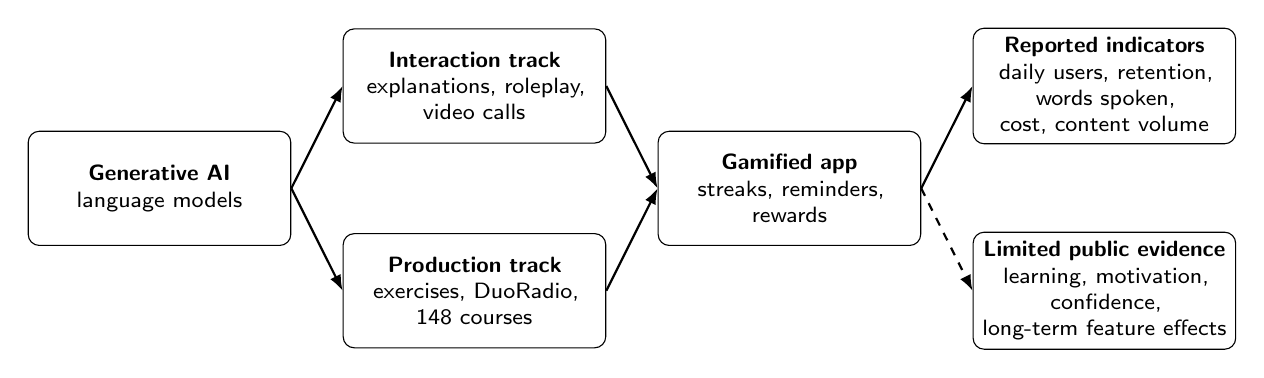
\begin{tikzpicture}[
box/.style={draw,rounded corners,align=center,text width=3.1cm,minimum height=1.45cm,font=\sffamily\footnotesize,execute at begin node={\hyphenpenalty=10000\exhyphenpenalty=10000}},
flow/.style={-{Latex[length=2mm]},thick}]
\node[box] (genai) at (0,0) {\textbf{Generative AI}\\language models};
\node[box] (interact) at (4,1.3) {\textbf{Interaction track}\\explanations, roleplay,\\video calls};
\node[box] (produce) at (4,-1.3) {\textbf{Production track}\\exercises, DuoRadio,\\148 courses};
\node[box] (app) at (8,0) {\textbf{Gamified app}\\streaks, reminders,\\rewards};
\node[box] (measured) at (12,1.3) {\textbf{Reported indicators}\\daily users, retention,\\words spoken,\\cost, content volume};
\node[box] (rare) at (12,-1.3) {\textbf{Limited public evidence}\\learning, motivation,\\confidence,\\long-term feature effects};
\draw[flow] (genai.east) -- (interact.west);
\draw[flow] (genai.east) -- (produce.west);
\draw[flow] (interact.east) -- (app.west);
\draw[flow] (produce.east) -- (app.west);
\draw[flow] (app.east) -- (measured.west);
\draw[flow,dashed] (app.east) -- (rare.west);
\end{tikzpicture}
\visualnote{Authors' synthesis of Tables~\ref{tab:timeline}--\ref{tab:ledger}. Solid output arrow: reported indicators; dashed: limited public evidence. Arrows do not establish causation or internal optimisation priorities. AI = artificial intelligence.}
\end{figure*}

\subsubsection{The Case for Enrichment}
The interaction workflows in Figure~\ref{fig:workflows} explain the strongest case for enrichment: responsive conversation and contextual explanations add ways to practise. Wider access potentially extends these opportunities \parencite{explainAccess2025,earnings2026}. Field-level findings make benefits plausible, but do not establish effects for Duolingo users \parencite{saarela2026}.

Human expertise also remains visible. Learning Designers write prompts and evaluation criteria and select generated content \parencite{contentProduction,duoradio}. A learning-design commentator describes the course expansion as a move towards human--AI collaboration, in which designers become orchestrators and quality guardians, and argues that it can combine scale through technology with quality through human expertise \parencite{hardman2025}. The expansion also added beginner courses for many language pairs that were not previously offered \parencite{courses2025}.

Video Call carries learner facts into later conversations, offering a route to contextual tailoring \parencite{henry2025}. The respondents surveyed by \textcite{catalan2026} wanted work-related scenarios, but their views do not establish that this feature supplies those scenarios. Access also remains tiered: Video Call is offered through paid subscriptions \parencite{earnings2026}.

\subsubsection{The Case for Industrialisation}
Figure~\ref{fig:duoradio-scale} separates the reported expansion in content supply from the increase in listening-session activity. Neither measure establishes an improvement in listening proficiency.

\begin{figure*}[t]
\caption{Company-Reported Expansion of DuoRadio Content and Use}
\label{fig:duoradio-scale}
\centering
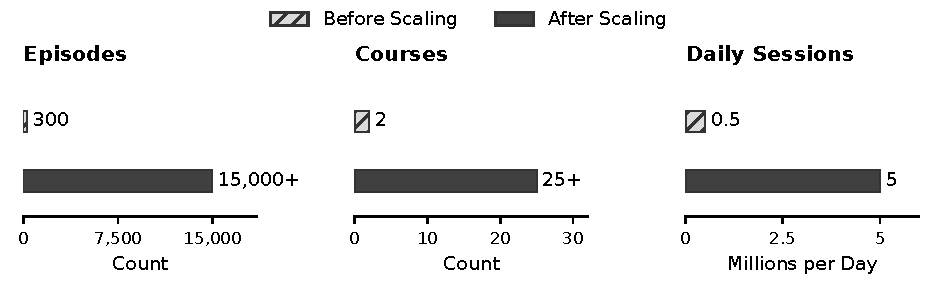
\includegraphics[width=\textwidth]{figures/duoradio-scale.pdf}
\visualnote{Original chart of company-reported figures \parencite{duoradio}. Bars labelled ``+'' end at the stated lower bound. Panels have different scales. Exact endpoint dates and listening-proficiency comparisons are not provided.}
\end{figure*}

The production accounts emphasise speed, volume, and cost. Figure~\ref{fig:duoradio-scale} shows the scale of DuoRadio expansion; the same account reports a 99\% cost saving \parencite{duoradio}. Management contrasts roughly twelve years for its first 100 courses with one year for nearly 150 \parencite{malikTechcrunch2025}, and links cheaper calls to wider subscription access \parencite{earnings2026}. Figure~\ref{fig:workflows} also shows the shift from writing exercises to specifying and selecting model output.

The inspected accounts of the 148 courses do not compare learning outcomes with earlier human-authored courses. The small learner-side study could not verify which lessons were generated \parencite{catalan2026}. Its respondents' request for work-relevant scenarios is consistent with the limitations of standardised content, but does not establish that generation caused them. External commentators question quality and evaluation priorities: \textcite{toczauer} highlights contextual relevance, cultural appropriateness, alignment with learning objectives, and the risk of prioritising engagement over learning; \textcite{hardman2025} likewise calls for guardrails. Reported social-media criticism raises similar concerns \parencite{malikTechcrunch2025}, but neither commentary nor user complaints constitute a quality measurement.

\subsubsection{Whose Outcomes Is the System Optimised For?}
The notification algorithm optimised a lesson-completion reward and reported gains in daily users and retention \parencite{yancey2020}. This establishes the objective of one pre-generative component. Two interpretive works raise the question of whether gamification mechanisms encourage dependence rather than autonomy: an eight-week design observation \parencite{maass2026} and a conceptual essay drawing on self-determination theory \parencite{espinosa2026}. Both raise a testable hypothesis rather than support a causal claim; neither followed a learner cohort or measured dependency. In a six-month study of 601 beginners, perseverance of effort and age predicted attrition \parencite{sudina2025}, indicating that continued use also varies with learner characteristics.

Autonomy is consequently an open evaluation question. A broad AI review associates independence with explicit self-regulation instruction and scaffolding \parencite{mohebbi2025}. Whether skills persist when cues or generated suggestions are withdrawn is a testable hypothesis, not an observed dependency outcome.

Management explicitly names better teaching and audience growth as priorities \parencite[letter p.~4]{shareholderQ12026}, and company studies do evaluate learners. Public disclosures reveal selected results and stated aims; they cannot establish how frequently unpublished outcomes are measured or how internal objectives are weighted.

\subsubsection{An Answer to RQ3}
Generative AI both expands practice capabilities and industrialises production and delivery. Lower costs are linked in company reporting to wider access, connecting the two. Demonstrated learner benefits remain unevenly supported. Operational and activity indicators are more extensively documented in this purposively selected public record than independent, long-term benefits; source selection may contribute to that asymmetry.

\clearpage
\section{Conclusion and Discussion}
\label{sec:conclusion-discussion}
\subsection{Conclusion}
Generative AI transforms the Duolingo user experience in two ways at once. It adds new kinds of interaction, in which learners obtain reasons for their errors and hold open conversations, and it changes how content is produced, so that far more courses and listening episodes can be created quickly and cheaply. The gamified, adaptive structure of the app remains in place, and both changes operate within it.

For RQ1, the features deployed since 2023 are Explain My Answer and Roleplay (March 2023) and Video Call (announced in September 2024), with wider access to Explain My Answer and Video Call in 2026, alongside generative production of lesson exercises (described in June 2023), DuoRadio episodes (scaled in 2024), and 148 new courses (April 2025). They differ from the pre-generative experience by adding generated contextual explanations and open conversation to existing feedback and exercise formats, while the production changes remain largely invisible to learners.

For RQ2, field-level research reports positive but heterogeneous effects. The direct Duolingo evidence is short-term and mostly company-authored. Selected users improved on some self-efficacy items; the Japanese study reported a speaking advantage, stable willingness to communicate, and neutral post-use confidence perceptions. Aggregate speech volume increased, but it cannot isolate a feature effect. A central finding is that no inspected study directly tests motivation effects of a confirmed generative feature, and emotional and cognitive engagement remain unmeasured. These findings do not establish a common confidence effect or durable benefit across users.

For RQ3, capability enrichment is documented through added conversation, explanations, and access, while industrialisation is documented through reported speed, volume, and cost. Demonstrated learner benefits are a separate, unevenly supported proposition. Operational and activity indicators are more extensively documented than independent, durable learner benefits in this selection. The review cannot determine Duolingo's internal optimisation priorities.

\subsection{Discussion}
\subsubsection{Interpretation}
Cheaper generation may be consequential because it can extend practice to more learners and language pairs. Limited positive learner findings support further evaluation, but do not settle generated-content quality, long-term transfer, or effects among users who discontinue practice. The review's contribution is to make those evidential differences visible alongside the dated changes. Reported efficiency is compatible with educational improvement; neither confirms the other.

For a practising Applied AI professional, the implication is that cost, throughput, and activity indicators are the easiest metrics to produce but the least informative about whether a feature works as intended. A product can report growing daily users, falling per-call costs, and rising word counts while the educational question --- whether learners acquire durable, transferable skill --- remains unanswered. Designing evaluations that measure learning, not just usage, is itself a professional competence this case illustrates.

\subsubsection{Reliability}
Dated releases, source locators, and the complete cited-source register make individual claims traceable. The register is retrospective, however: unrecorded search decisions cannot be reproduced, and no independent human duplicate extraction was conducted. Purposive selection may favour accessible company material and therefore amplify the apparent reporting asymmetry. The finding concerns this inspected record, not the prevalence of evidence across the entire literature. Live pages can change, limiting exact replication; retrieval dates and historical logs identify the version checked where available.

Abstract-only and indexed access prevent full appraisal of allocation, instruments, and uncertainty in several sources. These findings receive narrower interpretations, and unresolved details are recorded rather than filled from secondary annotations. Multiple company summaries may overlap, as may the primary studies within reviews; treating each citation as independent confirmation would exaggerate support.

\subsubsection{Validity}
Exposure, authorship, and outcome coding reduce claim--evidence mismatch but cannot repair the designs of the included studies. Adherence requirements and differential exclusions may select learners who tolerate or benefit from a feature; their outcomes cannot be generalised to everyone offered it. Post-use confidence perceptions do not estimate change, and non-significant findings do not establish no effect. Short follow-up and practised-phrase tests also limit claims about durable, unrehearsed communication.

Capability enrichment and industrialisation are an interpretive framework, not validated scales. Other framings could emphasise affordability or accessibility. Public reporting cannot disclose internal objective weights, and absent evidence in this review is not proof that no evaluation exists or that outcomes are poor. These limits constrain the answer to RQ3 rather than merely qualifying an otherwise certain priority ranking.

\subsubsection{Usability}
The paper can be used by educators deciding whether and how to recommend Duolingo, by learners interpreting the app's claims, and by developers and researchers planning evaluations. Educators can use the evidence map to decide which claims about AI features to relay to students and which to withhold pending stronger evidence. Learners can treat the paper as a reminder that completing a call or a streak does not by itself demonstrate proficiency, and that testing oneself outside the app remains the most informative check. Developers and researchers can use the gap analysis to design studies that fill the motivation and engagement voids identified here. The paper is not a product ranking and cannot predict how an individual learner will benefit.

\subsubsection{Recommendations}
\emph{Independent researchers}, with developer cooperation where needed, should prioritise a preregistered comparison of a named feature/version with regular lessons under comparable practice-time conditions. It should measure unrehearsed speaking with blinded scoring, validated self-efficacy and willingness-to-communicate scales separately, and delayed follow-up. Reporting all assigned learners, missing outcomes, and reasons for discontinuation would address the current adherence bias. This is a proposed study, not work completed here.

\emph{Duolingo and similar developers} should publish a versioned evaluation of generated explanations and lessons using sampled outputs, explicit accuracy and pedagogical-relevance criteria, and human adjudication. Comparing matched generated and earlier content on learner transfer would test whether the reported production gains preserve educational quality. Sampling rules, error denominators, and model/prompt versions should accompany the results.

\emph{Educators and learners} can meanwhile use generative interaction as additional practice and periodically assess progress on an unrehearsed conversation outside the app. Recording perceived capability separately from task performance would help identify when confidence and demonstrated progress diverge, without treating a streak or completed call as a proficiency measure.

\subsubsection{Transparency}
Generative AI tools assisted with source retrieval, organisation, and drafting. The authors are responsible for checking the cited sources and for the content of the paper.

\clearpage
\section*{References}
\addcontentsline{toc}{section}{References}
\printbibliography[heading=none]
\end{document}
